\section{Results}\label{sec:results}
The controllers have been implemented and tested on the quadcopter. Experimental results are shown for the attitude controller and simulation results are presented for the translational controllers. The latter includes the network and the non-linear system models simulated in MATLAB Simulink.

The obtained model parameters can be seen in \autoref{ParametersQuadcopter}. 
\begin{table}[H]
    \centering
    \begin{tabular}{|c|c|c|}
    \hline
        %------------------------------------------------------------------------------------------
        \textbf{Symbol} &\textbf{Value} &\textbf{Units}\\
        \hline %-----------------------------------------------------------------------------------
        $m$ & 0.996       &kg\\
        \hline %-----------------------------------------------------------------------------------
        $L$  &   0.225       & m\\
        \hline %-----------------------------------------------------------------------------------
        $J_x$  & 0.01073       & \si{kg \  m^2}\\
        \hline %-----------------------------------------------------------------------------------
        $J_y$  & 0.01073       & \si{kg \  m^2}\\
        \hline %-----------------------------------------------------------------------------------
        $J_z$  & 0.02135       & \si{kg \  m^2}\\
        \hline %-----------------------------------------------------------------------------------
        $k_{\mathrm{th}}$  & $1.32922\cdot10^{-5}$       & \si{N s^2 rad^{-2}}\\
        \hline %-----------------------------------------------------------------------------------
        $k_{\mathrm{d}}$  & $9.39741 \cdot10^{-7}$       & \si{N m s^2  rad^{-2}}\\
        \hline %-----------------------------------------------------------------------------------
        $\overline{\omega}_i$& 429      & \si{rad \ s^{-1}}\\
        \hline
    \end{tabular}
    \caption{Parameters used through the analysis and design.}
    \label{ParametersQuadcopter}
\end{table}
The mass and the length have been measured. $k_{\mathrm{th}}$ and $k_{\mathrm{d}}$ have been obtained by testing the propellers at different speeds. The moments of inertia have been calculated analytically by considering the quadcopter as a combination of different masses with known moments of inertia.\\
The value of delay used in the simulation is \fxnote{WRITE NUMBER} milliseconds and the missed packets probability is set to zero.\\
The attitude controller is defined by the designed $\vec{Q}$ and $\vec{R}$ diagonal matrices, shown below, and the chosen observer poles, which are $[-11, -12, -13]$.
%\footnotesize{
%\begin{flalign}   \label{Fematrix}
%	\vec{F}&=
%	\begin{bmatrix}
%		 0.00    & -165.15 & -223.35  &  0.00   &-44.04 & -68.52  \ \ \ \\
%		 165.15  &  0.00   & 223.35   &  44.04  & 0.00  &  68.52  \ \ \ \\
%		 0.00    & 165.15  & -223.35  &  0.00   &44.04  & -68.52  \ \ \ \\
%		 -165.15 & 0.00    & 223.35   & -44.04  & 0.00  &  68.52  \ \ \ 
%	\end{bmatrix}\nonumber\\
%		\vec{F}_{\mathrm{int}}&=
%		\begin{bmatrix}
%		   0.00   & -220.97 & -250.00  \ \ \ \\
%		   220.97 &   0.00  & 250.00   \ \ \ \\
%		   0.00   & 220.97  & -250.00  \ \ \ \\
%		  -220.97 &  0.00   &  250.00  \ \ \ 
%		\end{bmatrix}\nonumber
%\end{flalign}}
%\normalsize
\begin{center}
\noindent$\vec{Q}=diag\left(\frac{1}{0.2^2},\frac{1}{0.2^2},\frac{1}{0.1^2},\frac{1}{0.5^2},\frac{1}{0.5^2},\frac{1}{0.3^2},\frac{1}{0.08^2},\frac{1}{0.08^2},\frac{1}{0.05^2}\right)$

\noindent$\vec{R}=diag\left(\frac{1}{25^2},\frac{1}{25^2},\frac{1}{25^2},\frac{1}{25^2}\right).$
\end{center}

The controllers for $\dot{x}_{\mathrm{I}}$, $\dot{y}_{\mathrm{I}}$, $\dot{z}_{\mathrm{I}}$, $x_{\mathrm{I}}$, $y_{\mathrm{I}}$ and $z_{\mathrm{I}}$ are
\begin{minipage}{0.45\linewidth}
	\begin{flalign}
		C_{\dot{x}_{\mathrm{I}}}=-C_{\dot{y}_{\mathrm{I}}}=-0.0038\left(\frac{1+20s}{s}\right),\nonumber
	\end{flalign}
\end{minipage}   \hfill 
\begin{minipage}{0.45\linewidth}
		\begin{flalign}
		C_{x_{\mathrm{I}}}=C_{y_{\mathrm{I}}}=0.3,	\nonumber
	\end{flalign}
\end{minipage}\\

\begin{minipage}{0.45\linewidth}
		\begin{flalign}
		C_{\dot{z}_{\mathrm{I}}}=-201.8\left(\frac{s+0.8}{s}\right),\nonumber
	\end{flalign}
\end{minipage}   \hfill 
\begin{minipage}{0.45\linewidth}
	\begin{flalign}
		C_{z_{\mathrm{I}}}=1 .\nonumber
	\end{flalign}
\end{minipage}\\

These controllers are discretized using the Tustin method with a sampling time of \SI{35}{ms}. This is the minimum time in which data can be acquired from the motion tracking system, transmitted to and read by the microcontroller.

Figure \autoref{fig:pitchref} shows the attitude controller response when tracking a reference in the pitch angle.
\begin{figure}[H]
	\centering
	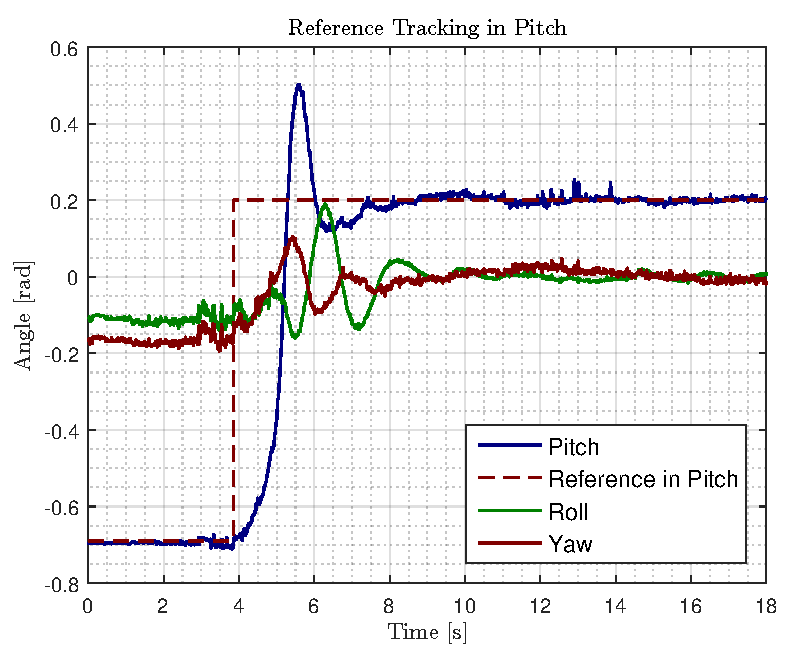
\includegraphics[width=.4\textwidth]{figures/pitchRefAcceptAllAngles}
	\caption{Attitude control response when tracking a reference in pitch.}
	\label{fig:pitchref}
\end{figure}

In \autoref{fig:positionControl}, the simulated step responses of the translational controllers along the three axes are depicted.
\begin{figure}[H]
	\centering
	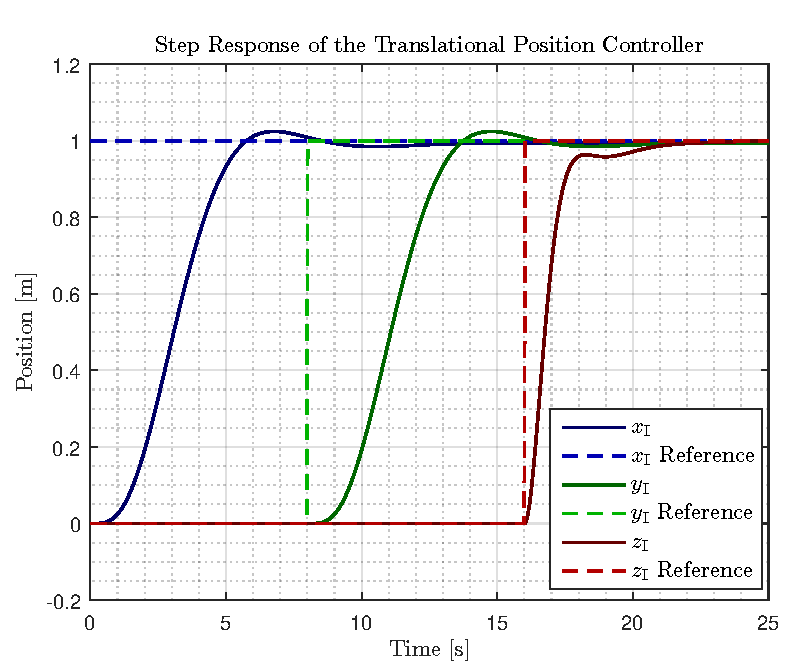
\includegraphics[width=.4\textwidth]{figures/stepTrans}
	\caption{Position control response in the three inertial axes. }
	\label{fig:positionControl}
\end{figure}
%
%The inner attitude controller results are also included and shown in \autoref{AttitudeControl} so the performance of the attitude control can be evaluated. 
%\begin{figure}[H]
%	\centering
%	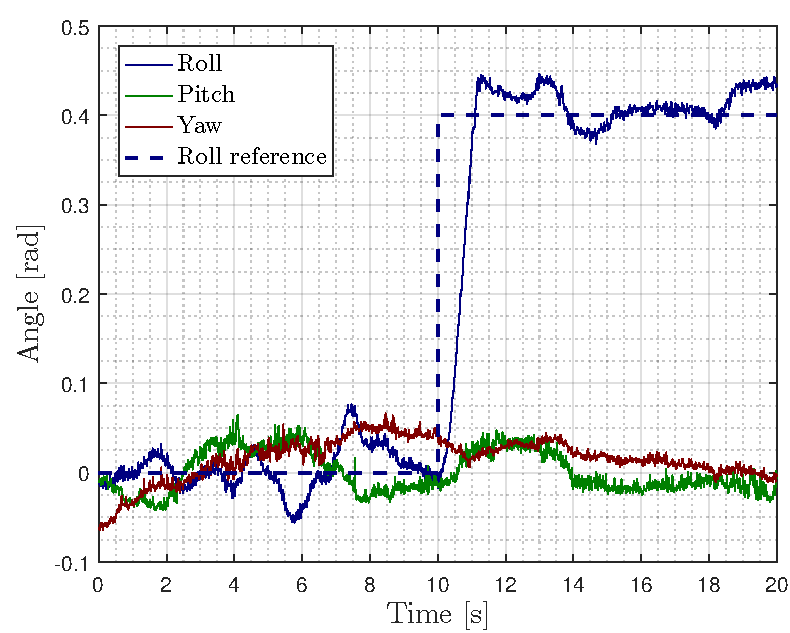
\includegraphics[width=.4\textwidth]{figures/AttitudeControl}
%	\caption{Attitude control results in the three angles. The references given to the attitude control system are shown with dashed lines.}
%	\label{AttitudeControl}
%\end{figure}